\section*{Exercise Part (B) - Generate RISC Code for The Chacha20 Stream Cipher}

\begin{enumerate}[wide, label=(B\arabic*)]

% (B1) Create an excel timing-diagram for the un-optimized RISC code, of the first 3 lines of the QUARTER-ROUND operation. Use the 7-stage pipeline in part B. You may assume that a register (say R0) contains the address of the first word of the block. (Your RISC code in parts B1 to B4 should show how all memory addresses are calculated, so use explicit memory addresses in your RISC instructions, ie LOAD R1,0(R0), where the memory address is 0+R0).
% • Highlight any assumptions that you make. Use a label, ie “ASSUMPTION #1” and explain it.
\item The unoptimized RISC code for the first 3 lines of the QUARTER-ROUND operation is shown in Listing~\ref{list:b1}. The following assumptions are made for this RISC code:
\begin{itemize}
	\item ASSUMPTION 1: assume that register R0 contains the address of the first word of the block of the initial key-stream
	\item ASSUMPTION 2: each word is 32 bits, so use LD and SD instead of LW and SD to load 32-bit words
	\item ASSUMPTION 3: words in the initial key-stream are stored consecutively in memory, address of second word is address of first world + 4 (bytes)
	\item ASSUMPTION 4: assume dual-ported memory that allows simultaneous read+read, read+write, write+write
\end{itemize}
\lstinputlisting[caption=Unoptimized RISC code for the first 3 lines of QUARTER-ROUND operation,label=list:b1,firstline=5]{../assembly/b1.s}
The timing diagram can be seen in Figure~\ref{fig:B1}. % need to figure out delay for stall.

\begin{figure}[htp]
    \centering
    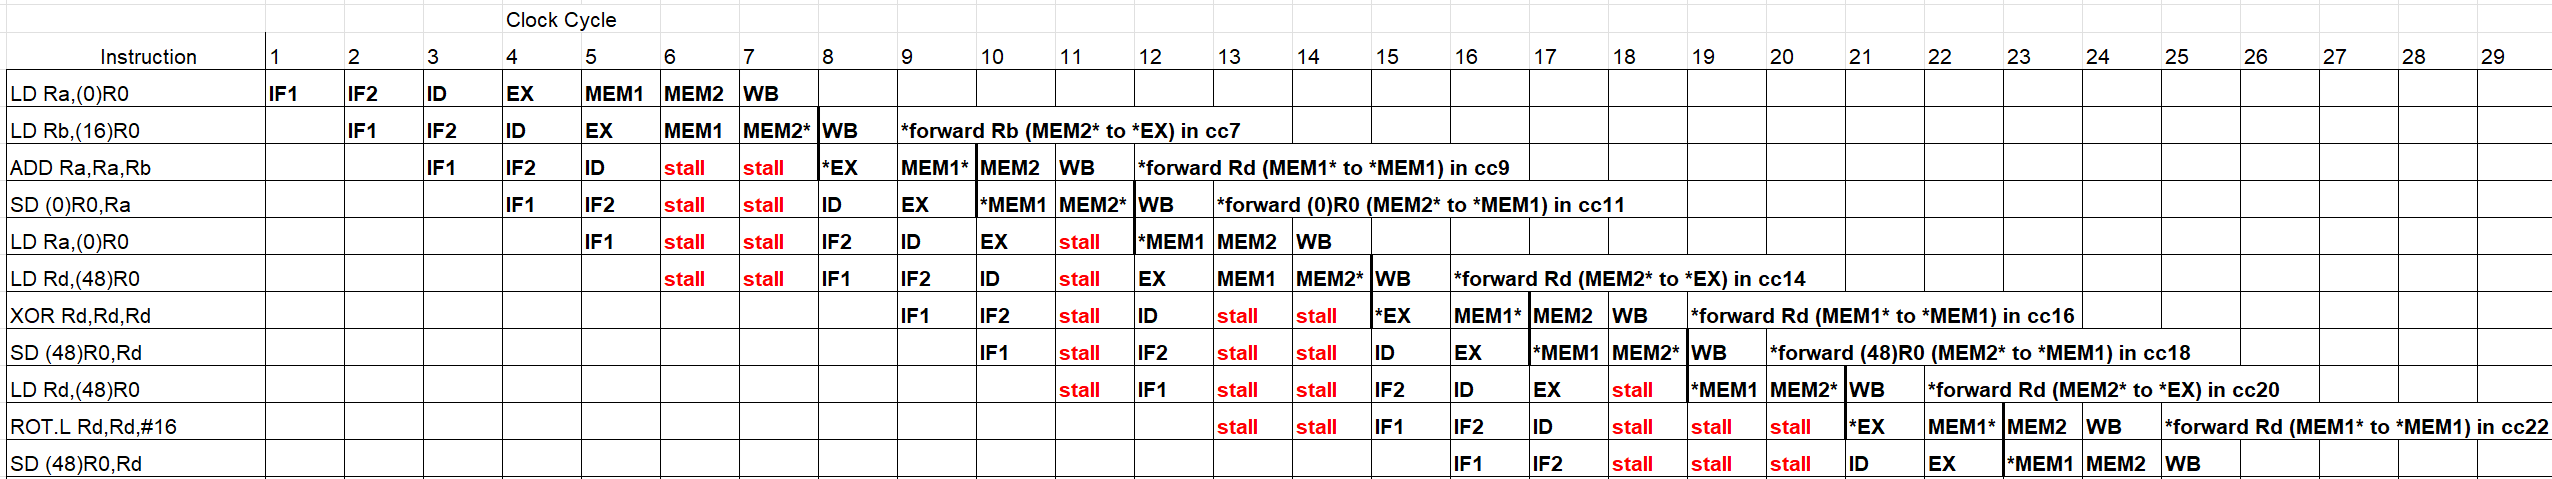
\includegraphics[width=\textwidth]{b1.png}
    \caption{\label{fig:B1}Timing Diagram for B1}
\end{figure}

% Write the un-optimized RISC code, for one QUARTER-ROUND operation (with 12 lines of C-code as shown in Fig. 2). (Use your insights gathered from B1.)
% Your answer can be a table with 3 columns: Column 1 is the RISC instruction. Column 2 is the number of stall cycles associated with that instruction. Column 3 can be a comment. You do not need to create a detailed timing-table.
% • Add a comment for every line of code. (Clear and concise comments take thought, and are worth marks.)
\item The unoptimized RISC code for one QUARTER-ROUND operation (along with the associated stall cycles per instruction) is shown in Table~\ref{tab:b2}. We make the same assumptions as we did in B1.


\begin{longtable}{|l|l|l|}
\caption{Unoptimized RISC code for QUARTER-ROUND operation}\label{tab:b2}\\

\hline \multicolumn{1}{|c|}{Instruction} &
\multicolumn{1}{c|}{Number of stall cycles} &
\multicolumn{1}{c|}{Comment} \\ \hline
\endfirsthead

\multicolumn{3}{c}%
{{\tablename\ \thetable{} -- continued from previous page}} \\
\hline \multicolumn{1}{|c|}{Instruction} &
\multicolumn{1}{c|}{Number of stall cycles} & 
\multicolumn{1}{c|}{Comment} \\ \hline
\endhead

\hline \multicolumn{3}{|r|}{{Continued on next page}} \\ \hline
\endfoot

\hline
\endlastfoot	

LD Ra,(0)R0	&0	& load a from memory  \\ \hline
LD Rb,(16)R0	&0	& load b from memory  \\ \hline
ADD Ra,Ra,Rb	&2	& a = a + b           \\ \hline
SD (0)R0,Ra	&2	& store a in memory   \\ \hline
LD Ra,(0)R0	&3	& load a from memory  \\ \hline
LD Rd,(48)R0	&3	& load d from memory  \\ \hline
XOR Rd,Rd,Rd	&3	& XOR(d,a)            \\ \hline
SD (48)R0,Rd	&3	& store d in memory   \\ \hline
LD Rd,(48)R0	&4	& load d from memory  \\ \hline
ROT.L Rd,Rd,\#16&5	& ROTATE\_LEFT(d, 16) \\ \hline
SD (48)R0,Rd	&3	& store d in memory   \\ \hline
LD Rc,(32)R0	&3	& load c from memory  \\ \hline
LD Rd,(48)R0	&3	& load d from memory  \\ \hline
ADD Rc,Rc,Rd	&2	& c = c + d           \\ \hline
SD (32)R0,Rc	&2	& store c in memory   \\ \hline
LD Rb,(16)R0	&3	& load b from memory  \\ \hline
LD Rc,(32)R0	&3	& load c from memory  \\ \hline
XOR Rb,Rb,Rc	&3	& XOR(b,c)            \\ \hline
SD (16)R0,Rb	&3	& store b in memory   \\ \hline
LD Rb,(16)R0	&4	& load b from memory  \\ \hline
ROT.L Rb,Rb,\#12&5	& ROTATE\_LEFT(b, 12) \\ \hline
SD (16)R0,Rb	&3	& store b in memory   \\ \hline
LD Ra,(0)R0	&3	& load a from memory  \\ \hline
LD Rb,(16)R0	&3	& load b from memory  \\ \hline
ADD Ra,Ra,Rb	&2	& a = a + b           \\ \hline
SD (0)R0,Ra	&2	& store a in memory   \\ \hline
LD Ra,(0)R0	&3	& load a from memory  \\ \hline
LD Rd,(48)R0	&3	& load d from memory  \\ \hline
XOR Rd,Rd,Rd	&3	& XOR(d,a)            \\ \hline
SD (48)R0,Rd	&3	& store d in memory   \\ \hline
LD Rd,(48)R0	&4	& load d from memory  \\ \hline
ROT.L Rd,Rd,\#8	&5	& ROTATE\_LEFT(d, 8)  \\ \hline
SD (48)R0,Rd	&3	& store d in memory   \\ \hline
LD Rc,(32)R0	&3	& load c from memory  \\ \hline
LD Rd,(48)R0	&3	& load d from memory  \\ \hline
ADD Rc,Rc,Rd	&2	& c = c + d           \\ \hline
SD (32)R0,Rc	&2	& store c in memory   \\ \hline
LD Rb,(16)R0	&3	& load b from memory  \\ \hline
LD Rc,(32)R0	&3	& load c from memory  \\ \hline
XOR Rb,Rb,Rc	&3	& XOR(b,c)            \\ \hline
SD (16)R0,Rb	&3	& store b in memory   \\ \hline
LD Rb,(16)R0	&4	& load b from memory  \\ \hline
ROT.L Rb,Rb,\#7	&5	& ROTATE\_LEFT(b, 7)  \\ \hline
SD (16)R0,Rb	&3	& store b in memory   \\ \hline
\end{longtable}

% (B3) Calculate the number of clock-cycles for the un-optimized QUARTER-ROUND in B2 to execute. (You can ignore the time to flush the pipeline.) Explain your answer clearly.
\item hi

% (B4) Optimize the QUARTER-ROUND code in B2, to minimize stalls. (The compiler will re- arrange instructions, to minimize stalls. The compiler will minimize the number of LOADs and STORES, to minimize stalls.) Create a compressed timing-diagram, to show how the QUARTER-ROUND will execute once it has been optimized. The timing-diagram will illustrate how many stalls occur. Explain how many clock cycles it takes, to execute the optimized QUARTER-ROUND operation.
% In the compressed timing diagram, use comments to indicate all forwarding of data and signals. A comment might be ‘* forward R0 (EX to D) in cc 7’. (If you have already made an uncompressed timing diagram, you can use that instead.)
\item hi again

\item 

\item 

\item 


\end{enumerate}